\documentclass[12pt, letterpaper]{article}
\usepackage[utf8]{inputenc}
\usepackage{graphicx}
\usepackage{hyperref}
\usepackage{fancyvrb}
\usepackage{array}
\usepackage{biblatex}
\usepackage{float}
\usepackage{subcaption}

\bibliography{rapport}

\title{Skin Cancer Detection Using Convolutional Neural Network}
\author{Komlan Jean-Marie DANTODJI
\\
    \multicolumn{1}{
        p{.7\textwidth}}{\centering\emph{Université Paris Vincennes St-Denis\\
  M1 Big Data\\}
  }
}
\date{\today}
\begin{document}


\begin{titlepage}
    \maketitle
\end{titlepage}

\tableofcontents

\newpage
\section{Introduction}
\par Skin cancer is a disease of human’s body which can be cured easily if it can be detected so early. Today the evolution of the artificial intelligence technology helps to detect cancerous cells responsible for skin cancer. \\
\subsection{Issue}
\par The problem here is to find a way to diagnostic whether an image of the skin contain cancerous cells or not. To get there we have choose the deep learning algorithm CNN (Convolutional Neuronal Network) which gives high accuracy. 
\subsection{Background and Related works}
\par Before dermatologist used to analyze the image of patients skin by locking for cancerous cells in the image. This way of detection reaches his limit whenever we are in front of huge images of patients. To automate the detection, \\
\begin{itemize}
		\item Robert Amelard et al:\\
		They suggested an illumination correction and feature extraction framework based on high level intuitive feature implemented on skin images.
		\item A. Goshtasbya D. Rosemanb S. Binesb C. Yuc A. Dhawand A. Huntleye L. Xua:\\
		They proposed an artificial neural network approach with Back-propagation neural network (BNN) and Auto-associative neural network.
		\item Ramteke et al. : \\
		They have proposed a method dependent on ABCD standard to recognize skin malignant growth
		\item Sibi Salim RB Aswin, J Abdul Jaleel. 2013: \\
		Implementation of ANN Classifier using MATLAB for Skin Cancer Detection.
\end{itemize}



\section{Dataset}

\par The input data here are images of patients’ skin taken with high resolution. This method use 23907 image collected from ISIC Archive. Images with cancerous cells are labeled malignant and benign for favorable images.

\section{Different step of detecting cancer in image} 
\begin{figure}[H]
    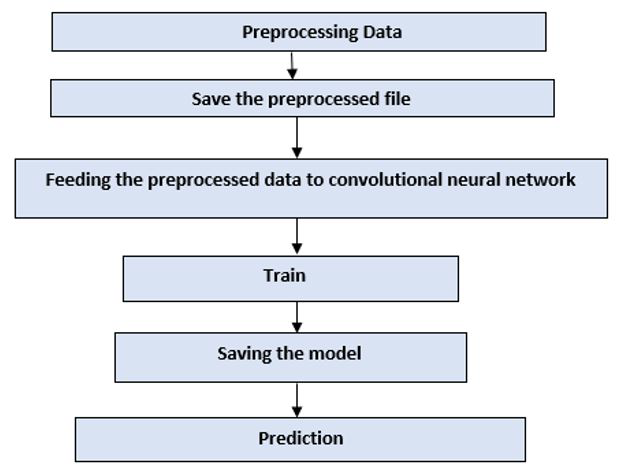
\includegraphics[width=\linewidth]{images/steps.png}
    \caption{[1] Chart display steps of the model CNN, page 255}
    \label{fig:L1}
\end{figure}
\subsection{Step 1: Preprocessing Data}
\par All images present in the dataset must be resized to the minimum size in other to reduce time of processing. The same process is made for the input image. After that, we have to convert the image from RGB color to gray scale.

\subsection{Step 2: Save the preprocessed file}
\par The images in dataset are classified to their class label: benign and malignant.
\subsection{Step 3: Feeding the preprocessed data to convolutional neuronal network (CNN)}
\par At this step assume we have an image of gray-scale of 6x6 and filter 3x3 we calculate the convolutional layer of each block of 3x3 by moving around the column and then the rows by using the formula followed:
$$ \sum_{i=0}^{m-1}\sum_{i=0}^{n-1} X_{(m-i)(n-j)}Y_{(i+1)(j+1)}$$
We get finally 4x4 image the pooling layer 
\begin{figure}[H]
    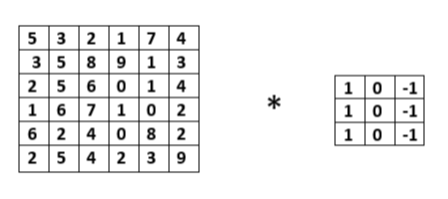
\includegraphics[width=\linewidth]{images/convolution.png}
    \caption{[1] Gray-scale Image 6x6 and the 3x3 filter, page 256}
    \label{fig:L1}
\end{figure}
After applying the convolutional formula we get the image as follow
\begin{figure}[H]
    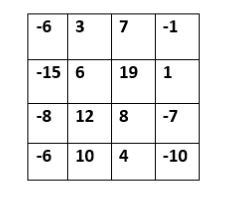
\includegraphics[width=7cm,height=6cm]{images/pooling.png}
    \caption{[1] 4x4 image after applying 3x3 filter to the gray-scale image, page 257}
    \label{fig:L1}
\end{figure}
To extract more complex feature we apply the max pooling which consist of getting the maximum of the consecutive 2x2 block from the pooling layer.
\begin{figure}[H]
    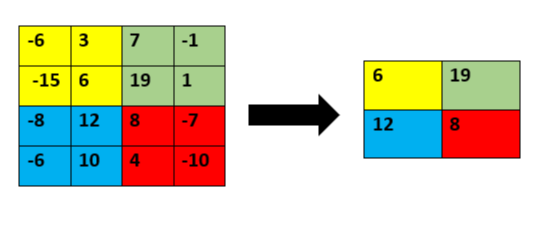
\includegraphics[width=\linewidth]{images/maxpooling.png}
    \caption{[1] Result after applying max pooling, page 257}
    \label{fig:L1}
\end{figure}
\subsection{Step 4: Train}
\par At this point we train the model 200 times of epoch.
\subsection{Step 5: Saving the model }
\par Here the model is saved for testing or predict whether a new input image belongs to the benign or malignant class.
\subsection{Step 6: Prediction}
\par At this last step we can feed images to our model for prediction. We evaluate the model by getting the accuracy, precision, recall and the score.
$$ Recall = \frac{TruePositive}{Positive }$$
$$ Specificity = \frac{TrueNegative}{Negative}$$
$$ Precision = \frac{TruePositive}{TruePositive + FalsePositive}$$
$$ Score = \frac{2*Precision*Recall}{Precision+Recall}$$


\section{Discussion} 
\begin{figure}[H]
    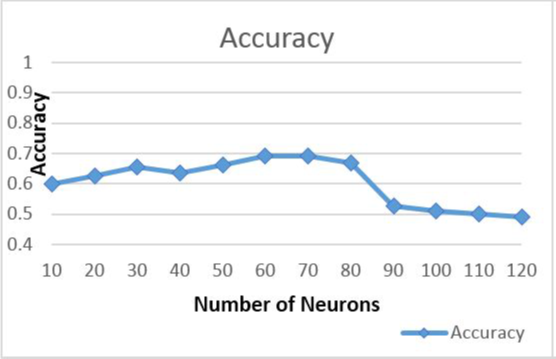
\includegraphics[width=12cm,height=6cm]{images/discuss_1.png}
    \caption{[1] Neurons vs accuracy, page 257}
    \label{fig:L1}
\end{figure} 
\begin{figure}[H]
    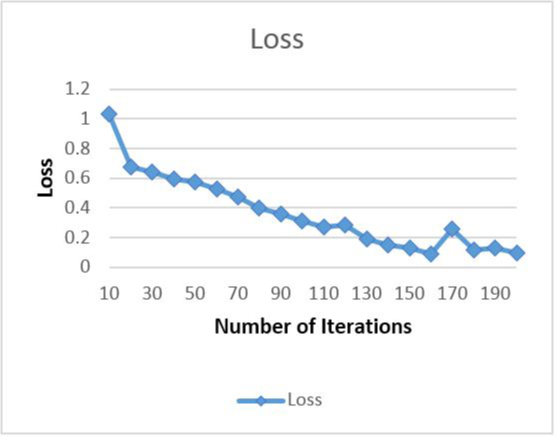
\includegraphics[width=12cm,height=6cm]{images/discuss_2.png}
    \caption{[1] Iteration vs loss, page 258}
    \label{fig:L1}
\end{figure} 
\begin{figure}[H]
    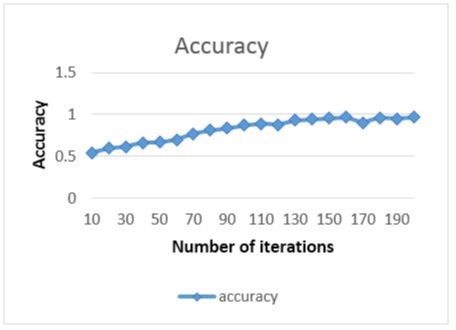
\includegraphics[width=12cm,height=6cm]{images/discuss_3.png}
    \caption{[1] Iteration vs accuracy, page 258}
    \label{fig:L1}
\end{figure} 
\begin{figure}[H]
    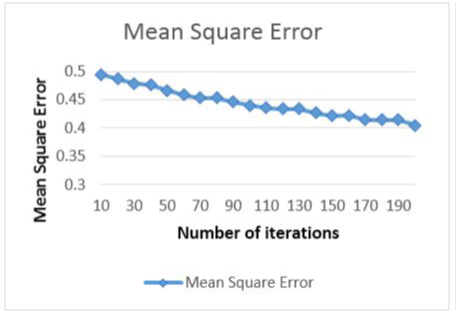
\includegraphics[width=12cm,height=6cm]{images/discuss_4.png}
    \caption{[1] Iteration vs Mean Square Error, page 258}
    \label{fig:L1}
\end{figure} 

\section{Results}
With this model using ISIC archive dataset we get the the result 
$$Recall = 0.84$$
$$Precision = 0.8325$$
$$Score = 0.8325$$
according to [1].

\newpage
\section{Conclusion}
\par This model is useful for dermatologist in their assistance to help for detection whether a patient have skin cancer or not. 
 


\section{Reférences}
\par [1] Mahamudul Hasan, Samia Islam, Surajit Das Barman, Ahmed Wasif Reza. Skin Cancer Detection Using Convolutional Neural Network published in the conference: the 2019 5th International Conference in April 2019.


\newpage
\printbibliography
\end{document}
